%-------------------------------------------------------------------------------
%	NAME:	report.tex
%	AUTHOR: Connor Beardsmore - 15504319
%	LAST MOD:	28/09/17
%	PURPOSE:	FCC Assignment Report
%	REQUIRES:	NONE
%-------------------------------------------------------------------------------

\documentclass[]{article}
\usepackage[ margin=3cm ]{geometry}
\usepackage{graphicx}
\usepackage{fancyhdr}
\usepackage{float}
\usepackage{hyperref}
\usepackage{transparent}
\usepackage{multicol}
\usepackage{amsmath}
\usepackage[final]{pdfpages}
\usepackage{listings}
\usepackage{color}

\pagestyle{fancy}
\fancyhf{}
\lhead{Connor Beardsmore - 15504319}
\rhead{FCC200}
\lfoot{April 2017}
\rfoot{\thepage}

\pagenumbering{arabic}
\graphicspath{{./images/}}

%-------------------------------------------------------------------------------
% CODE HIGHLIGHTING FOR LISTINGS
\definecolor{codegreen}{rgb}{0,0.6,0}
\definecolor{codegray}{rgb}{0.5,0.5,0.5}
\definecolor{codepurple}{rgb}{0.58,0,0.82}
\definecolor{backcolour}{rgb}{0.99,0.99,0.99}

\lstdefinestyle{mystyle}{
	backgroundcolor=\color{backcolour},   
	commentstyle=\color{codegreen},
	keywordstyle=\color{magenta},
	numberstyle=\tiny\color{codegray},
	stringstyle=\color{codepurple},
	basicstyle=\footnotesize,
	breakatwhitespace=false,         
	breaklines=true,                 
	captionpos=b,                    
	keepspaces=true,                 
	numbers=left,                    
	numbersep=5pt,                  
	showspaces=false,                
	showstringspaces=false,
	showtabs=false,                  
	tabsize=2
}

\lstset{style=mystyle}


%-------------------------------------------------------------------------------
\begin{document}
%-------------------------------------------------------------------------------
% TITLE PAGE

\begin{titlepage}
	\begin{center}
		\vspace*{1cm}
		\LARGE\textbf{FCC200 Report}
		\break
		Affine Cipher and S-DES Implementation
		\vspace{1cm}
		\break
		\Large\textbf{Connor Beardsmore - 15504319} 
		\vspace{15cm}

		\normalsize
		Curtin University \\
		Science and Engineering \\
		Perth, Australia \\
	    April 2017
	    
	\end{center}
\end{titlepage}

%-------------------------------------------------------------------------------
% AFFINE CIPHER

\vspace*{-0.8cm}
\begin{center}
	\section*{Affine Cipher}
\end{center}

\vspace*{0.8cm}
\subsection*{Compute Eligible Keys}

There are two keys required, \textit{a} and \textit{b}. The first is required to be \textit{coprime} with the length of the alphabet, in this scenario \textit{26}. The second key representing the linear shift must be both positive and less than the length of the alphabet. To check if the \textit{a} value is coprime, the following greatest common denominator check was utilized. If the greatest common denominator of \textit{a} and 26 is 1, the value of \textit{a} is \textit{coprime} and the key is valid in combination with any valid \textit{b} value.\\

\lstinputlisting[language=C,linerange={34-60} ]{../affine/keyeligible.c} 

\vspace{0.5cm}
The results of calling this function on all \textit{a} values from 1 to 25 are as follows:\\

\begin{multicols}{2}
	\begin{itemize}
		\item \textbf{gcdFunction( 1, 26 ) = 1}
		\item gcdFunction( 2, 26 ) = 2
		\item \textbf{gcdFunction( 3, 26 ) = 1}
		\item gcdFunction( 4, 26 ) = 2
		\item \textbf{gcdFunction( 5, 26 ) = 1}
		\item gcdFunction( 6, 26 ) = 2
		\item \textbf{gcdFunction( 7, 26 ) = 1}
		\item gcdFunction( 8, 26 ) = 2
	    \item \textbf{gcdFunction( 9, 26 ) = 1}
		\item gcdFunction( 10, 26 ) = 2
		\item \textbf{gcdFunction( 11, 26 ) = 1}
		\item gcdFunction( 12, 26 ) = 2
		\item gcdFunction( 13, 26 ) = 13
		\item gcdFunction( 14, 26 ) = 2
		\item \textbf{gcdFunction( 15, 26 ) = 1}
		\item gcdFunction( 16, 26 ) = 2
		\item \textbf{gcdFunction( 17, 26 ) = 1}
		\item gcdFunction( 18, 26 ) = 2
		\item \textbf{gcdFunction( 19, 26 ) = 1}
		\item gcdFunction( 20, 26 ) = 2
		\item \textbf{gcdFunction( 21, 26 ) = 1}
		\item gcdFunction( 22, 26 ) = 2	
		\item \textbf{gcdFunction( 23, 26 ) = 1}
		\item gcdFunction( 24, 26 ) = 2
		\item \textbf{gcdFunction( 25, 26 ) = 1}
	\end{itemize}
\end{multicols}


\vspace{0.5cm}

The full list of valid \textit{a} values is: \textbf{1, 3, 5, 7, 9, 11, 15, 17, 19, 21, 23, 25}\\

There are a total of 12 possible \textit{a} values that are coprime with \textit{26}. Each of these values can have a shift value (\textit{b}) of 0 to 25. Thus, the total number of eligible keys is:

$$12*26=312$$

Of these, 26 keys are trivial Caesar ciphers and 286 are non-trivial.

\subsection*{Recovered Plaintext}

\begin{figure}[H]
	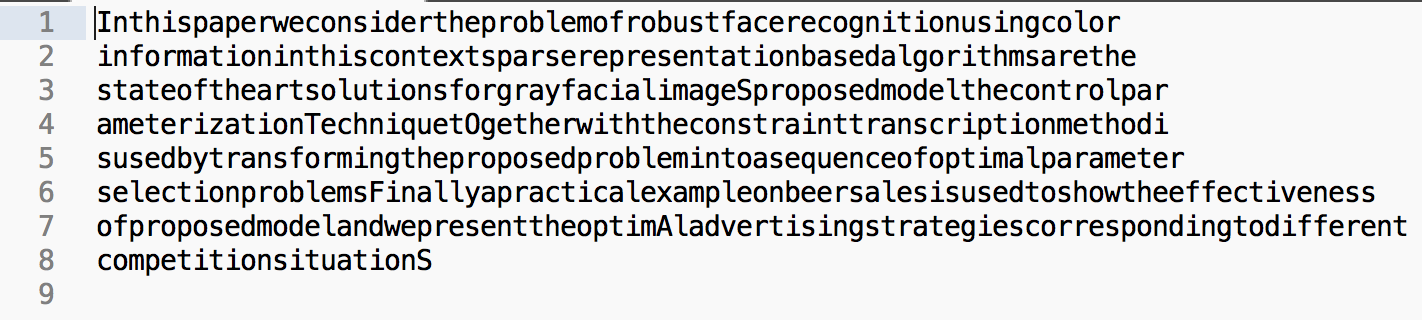
\includegraphics[width=\textwidth]{affine_plaintext.png}
	\caption{Original Plaintext File}
	\centering
\end{figure}

\begin{figure}[H]
	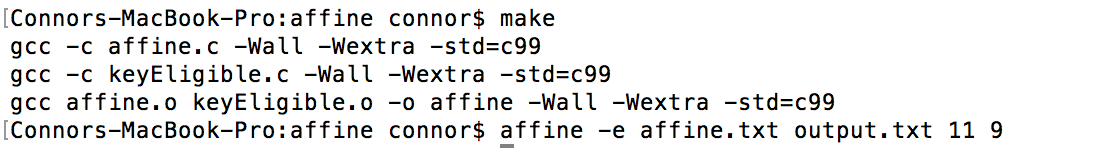
\includegraphics[width=\textwidth]{affine_encrypt.png}
	\caption{Encryption Process}
	\centering
\end{figure}

\begin{figure}[H]
	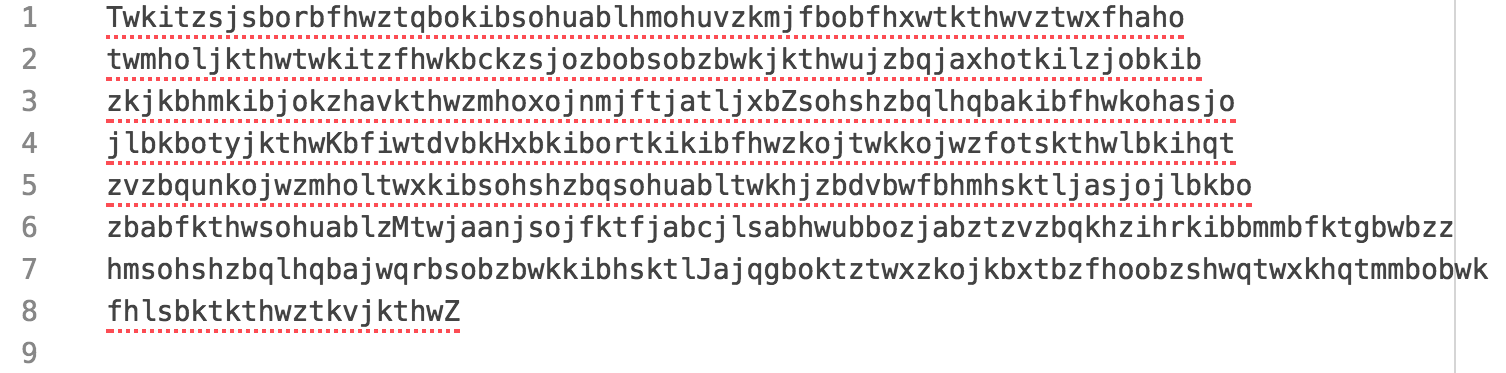
\includegraphics[width=\textwidth]{affine_ciphertext.png}
	\caption{Encrypted Ciphertext File}
	\centering
\end{figure}

\begin{figure}[H]
	
\includegraphics[width=\textwidth]{affine_decrypt.png}
	\caption{Decryption Process}
	\centering
\end{figure}

\begin{figure}[H]
d	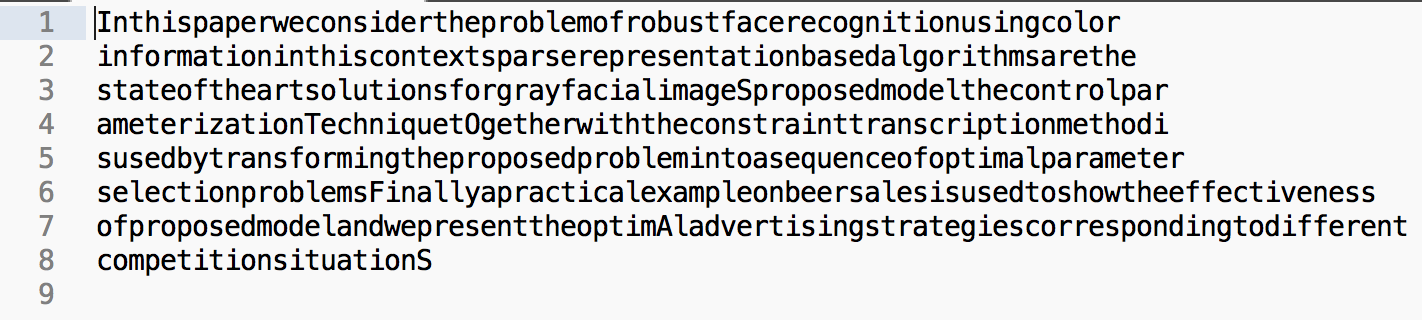
\includegraphics[width=\textwidth]{affine_plaintext.png}
	\caption{Recovered Plaintext file}
	\centering
\end{figure}

\subsection*{Affine Mathematical Proof}

The encryption and decryption functions for the affine cipher are as follows:

$$E(x)=(ax+b)\;mod\;m$$

$$D(x)=a^{-1}(x-b)\;mod\;m$$

\vspace{0.5cm}

The modular multiplicative inverse of \textit{a} is defined as:

$$1=aa^{-1}\;mod\;m$$

It can be shown that \textit{D(x)} is the inverse of \textit{E(x)} via the modular arithmetic laws.

\begin{equation*}
\begin{split}
D(E(x)) & = a^{-1}(E(x)-b)\;mod\;m \\
& = a^{-1}(( ax+b\;mod\;m )-b)\;mod\;m \\
& = a^{-1} (ax+b-b) \;mod\;m \\
& = a^{-1}ax\;mod\;m \\
& = x\;mod\;m
\end{split}
\end{equation*}




\subsection*{Letter Distribution}

For the given test file shown in Figure 2, the following table and Figure 7 illustrate the letter distribution and relative frequencies.

\begin{multicols}{7}
	\begin{itemize}
		\item A: 35
		\item B: 7
		\item C: 17
		\item D: 14
		\item E: 65
		\item F: 14
		\item G: 10
		\item H: 16
		\item I: 41
		\item J: 0
		\item K: 0
		\item L: 18
		\item M: 16
		\item N: 35
		\item O: 50
		\item P: 23
		\item Q: 2
		\item R: 39
		\item S: 39
		\item T: 53
		\item U: 8
		\item V: 2
		\item W: 4
		\item X: 2
		\item Y: 3
		\item Z: 1
	\end{itemize}
\end{multicols}

\begin{figure}[H]
	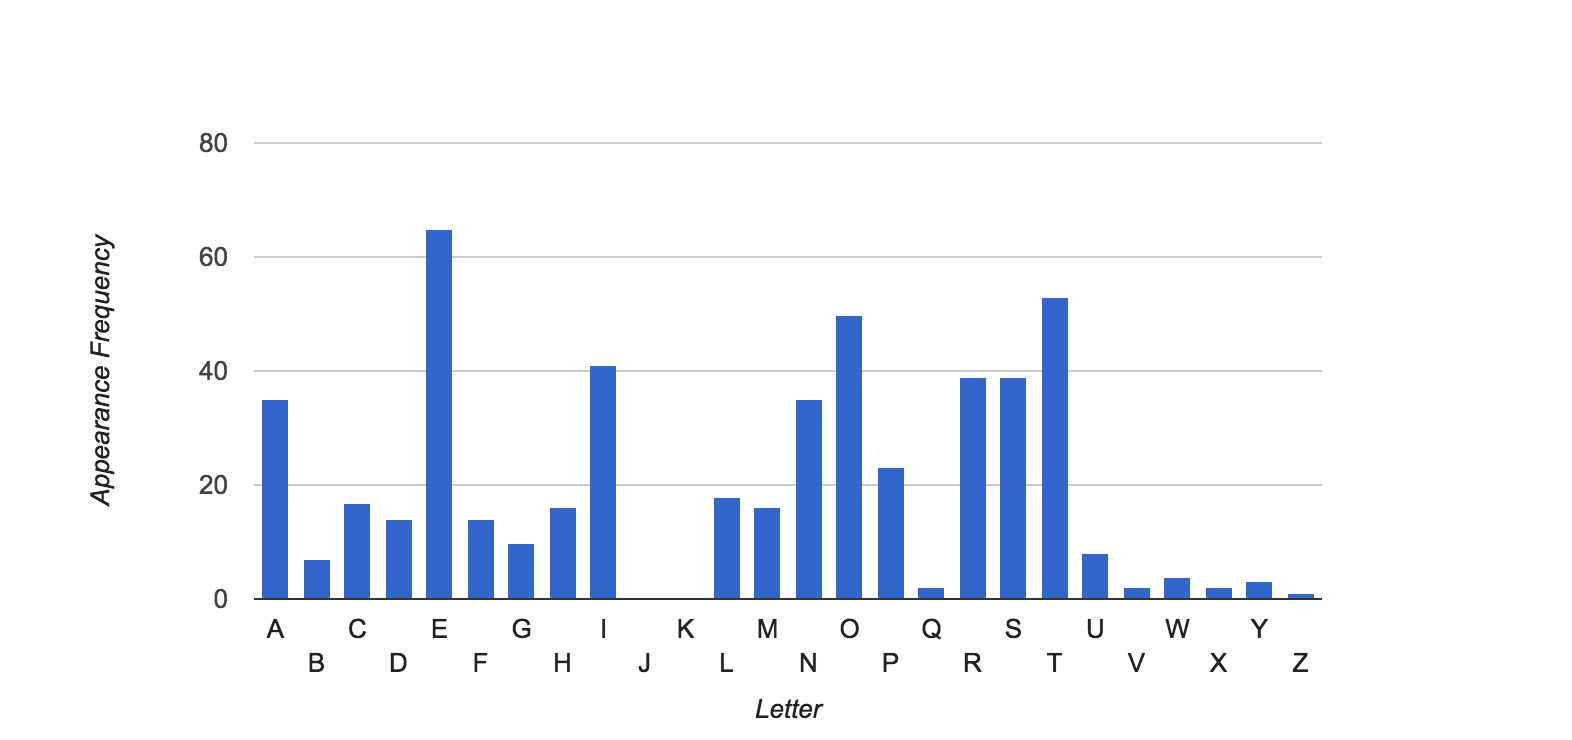
\includegraphics[width=\textwidth]{frequency.png}
	\caption{Letter Distributions}
	\centering
\end{figure}

\break
%-------------------------------------------------------------------------------
% S-DES ENCRYPTION

\vspace*{-0.8cm}
\begin{center}
	\section*{S-DES}
\end{center}

\vspace*{0.8cm}
\subsection*{S-DES Mathematical Proof}

hello

\subsection*{Pseudo Code Structure}

hello

\subsection*{Encrypted Test File}

\begin{figure}[H]
	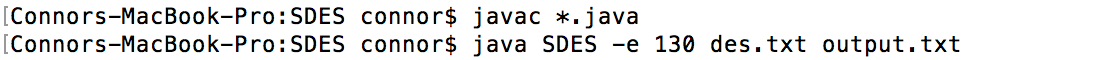
\includegraphics[width=\textwidth]{sdes_encrypt.png}
	\caption{S-DES Encryption Process}
	\centering
\end{figure}

\begin{figure}[H]
	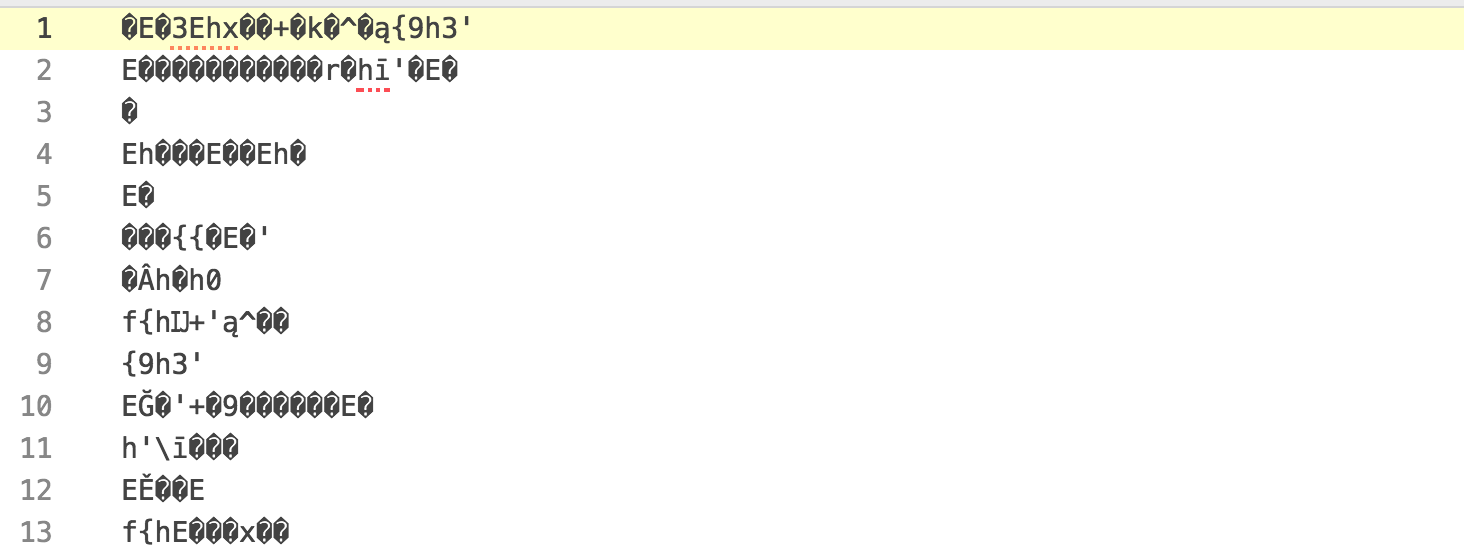
\includegraphics[width=\textwidth]{sdes_cipher1.png}
	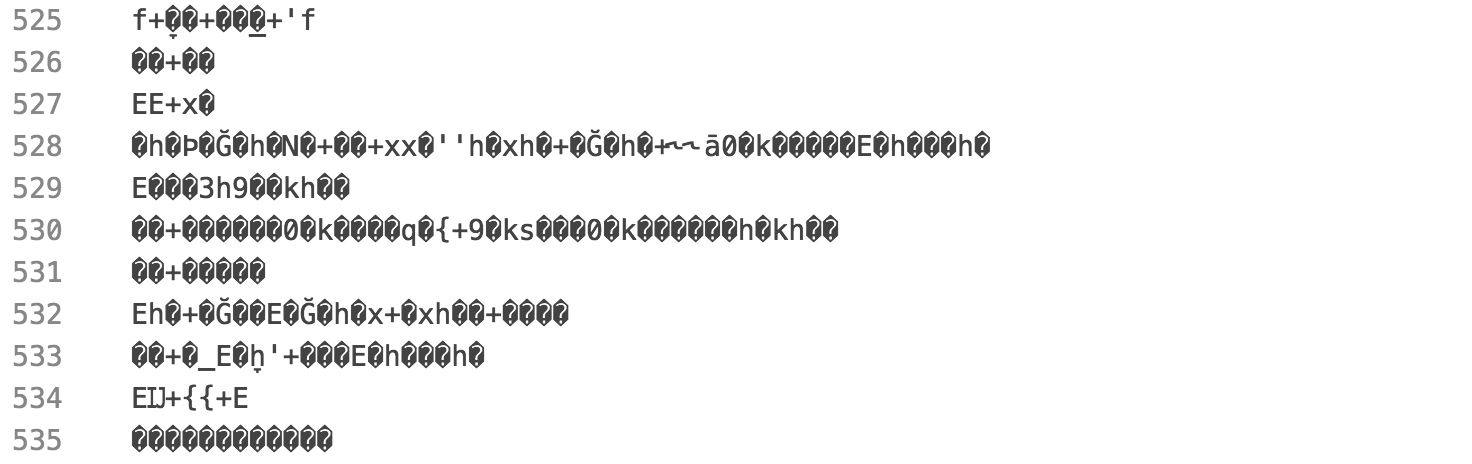
\includegraphics[width=\textwidth]{sdes_cipher2.png}	
	\caption{S-DES Cipher Text}
	\centering
\end{figure}

\subsection*{Decrypted Test File}

\begin{figure}[H]
	
\includegraphics[width=\textwidth]{sdes_decrypt.png}
	\caption{S-DES Decryption Process}
	\centering
\end{figure}

\begin{figure}[H]
	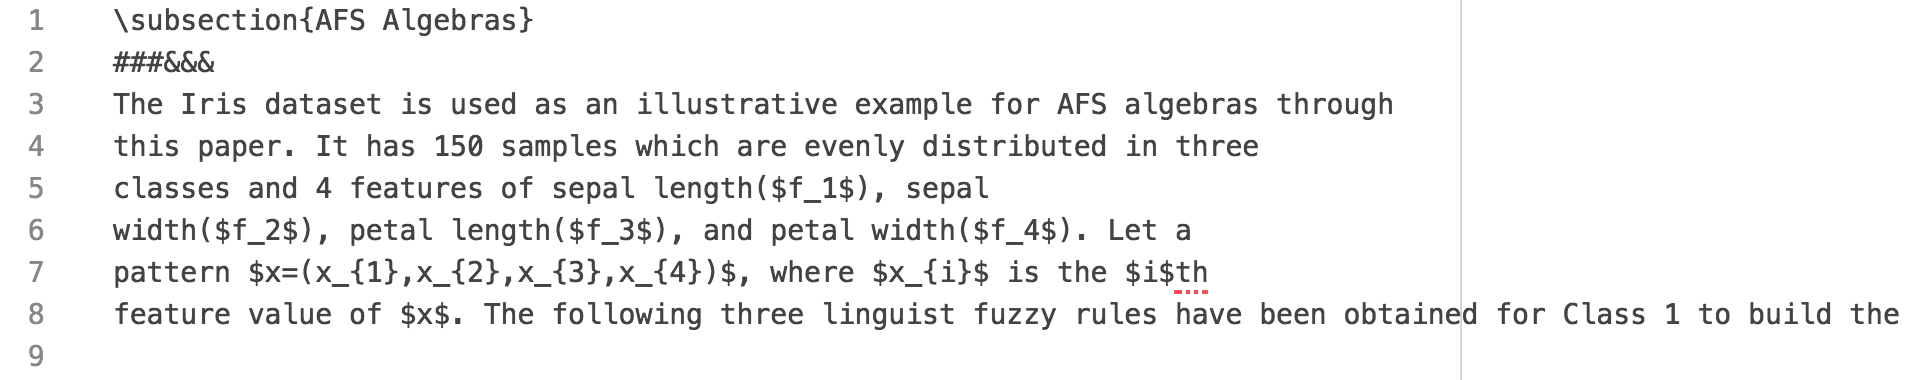
\includegraphics[width=\textwidth]{sdes_plain1.png}
	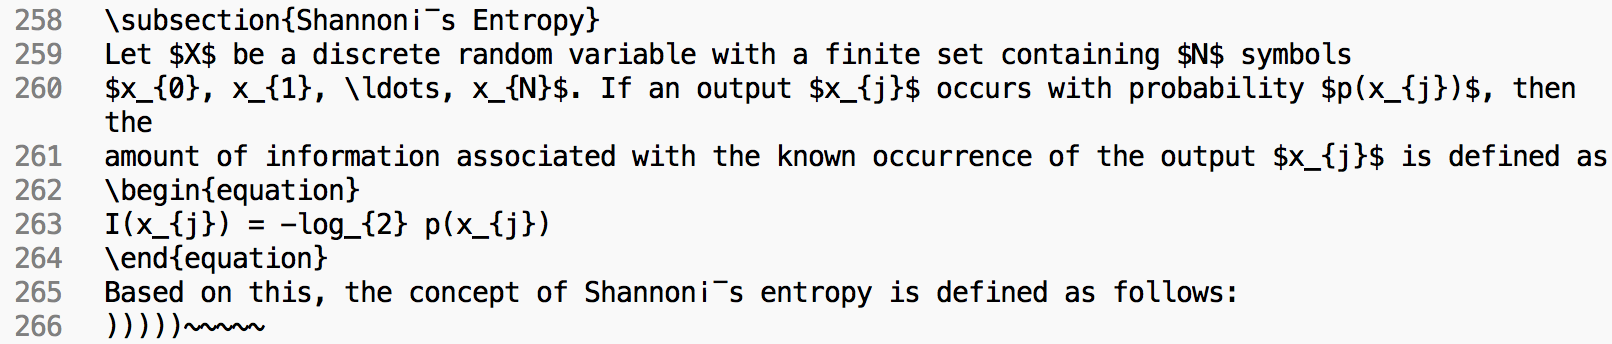
\includegraphics[width=\textwidth]{sdes_plain2.png}	
	\caption{S-DES Plain Text}
	\centering
\end{figure}

\subsection*{Utilization of an all 1 Key}

hello

\subsection*{Modify S-Boxes}

hello

\break
%-------------------------------------------------------------------------------
% FINAL QUESTIONS

\vspace*{-0.8cm}
\begin{center}
	\section*{Additional Questions}
\end{center}

\vspace*{0.8cm}
\subsection*{Threats}

hello \\

\subsection*{Source Coding}

Source coding in information transmission aims to compress natural messages for highly efficient message transfer.

\subsection*{Error Coding}

Error coding in information transmission attempts to enable a high information rate by the introduction of redundancy to data, as well as via error detection and correction mechanisms.

\subsection*{S-DES Coding}

hello \\

\subsection*{S-DES Confusion and Diffusion}

In S-DES, confusion is provided by the S-BOX substitutions performed within the feistal key round. Diffusion in contrast is provided by the permutations applied to the data included the expansion permutation utilized.

\pagebreak

%-------------------------------------------------------------------------------
% AFFINE CODE

\vspace*{-0.8cm}
\begin{center}
	\section*{Affine Source Code}
\end{center}

\subsection*{keyeligible.h}
\lstinputlisting[language=C,linerange={} ]{../affine/keyeligible.h}\pagebreak{}
\subsection*{keyeligible.c}
\lstinputlisting[language=C,linerange={} ]{../affine/keyeligible.c}\pagebreak{}
\subsection*{affine.h}
\lstinputlisting[language=C,linerange={} ]{../affine/affine.h}\pagebreak{}
\subsection*{affine.c}
\lstinputlisting[language=C,linerange={} ]{../affine/affine.c}\pagebreak{}

%-------------------------------------------------------------------------------
% SDES CODE

\vspace*{-0.8cm}
\begin{center}
	\section*{S-DES Source Code}
\end{center}

\subsection*{SDESConstants.java}
\lstinputlisting[language=java,linerange={} ]{../SDES/SDESConstants.java}\pagebreak{}
\subsection*{SDESBits.java}
\lstinputlisting[language=java,linerange={} ]{../SDES/SDESBits.java}\pagebreak{}
\subsection*{SDES.java}
\lstinputlisting[language=java,linerange={} ]{../SDES/SDES.java}\pagebreak{}

%-------------------------------------------------------------------------------
\end{document}   
%-------------------------------------------------------------------------------: